\documentclass[nonacm,sigconf,natbib=false]{acmart}

%%
%% \BibTeX command to typeset BibTeX logo in the docs
\AtBeginDocument{%
  \providecommand\BibTeX{{%
    Bib\TeX}}}

%%
%% The majority of ACM publications use numbered citations and
%% references, obtained by selecting the acmnumeric BibLaTeX style.
%% The acmauthoryear BibLaTeX style switches to the "author year" style.
%%
%% If you are preparing content for an event
%% sponsored by ACM SIGGRAPH, you must use the acmauthoryear style of
%% citations and references.
%%
%% Bibliography style
\RequirePackage[
  datamodel=acmdatamodel,
  style=acmnumeric,
  ]{biblatex}

%% Remove auto generated acm text
\setcopyright{none}
\settopmatter{printacmref=false} % Removes citation information below abstract
\renewcommand\footnotetextcopyrightpermission[1]{} % removes footnote with conference information in first column
\pagestyle{plain}

%% Declare bibliography sources (one \addbibresource command per source)
\addbibresource{linear_agreement_and_liveness.bib}

%%
%% end of the preamble, start of the body of the document source.
\begin{document}

%%
%% The "title" command has an optional parameter,
%% allowing the author to define a "short title" to be used in page headers.
\title{Liveness-Probleme durch Optimierungen in Konsensusprotokollen} % Original: Linear Agreement and Liveness 

%%
%% The "author" command and its associated commands are used to define
%% the authors and their affiliations.
\author{Eugen Becker}
\email{eugen.becker@fau.de}
\affiliation{%
  \institution{Friedrich-Alexander-Universität Erlangen-Nürnberg}
  \streetaddress{}
  \city{}
  \state{}
  \postcode{}
  \country{}
}

%%
%% By default, the full list of authors will be used in the page
%% headers. Often, this list is too long, and will overlap
%% other information printed in the page headers. This command allows
%% the author to define a more concise list
%% of authors' names for this purpose.
\renewcommand{\shortauthors}{Eugen Becker}

%% Change abstract heading to Kurzfassung
\renewcommand{\abstractname}{Kurzfassung}

%% Change the bibliography title
\renewcommand{\refname}{Bibliographie}

%%
%% The abstract is a short summary of the work to be presented in the
%% article.
\begin{abstract}
  To do ...

  To do ...

  To do ...

  To do ...

  To do ...

  To do ...

  To do ...

  To do ...

  To do ...

  To do ...

  To do ...

  To do ...
\end{abstract}

%%
%% Keywords. The author(s) should pick words that accurately describe
%% the work being presented. Separate the keywords with commas.
%%\keywords{Do, Not, Us, This, Code, Put, the, Correct, Terms, for,
%%  Your, Paper}

%%
%% This command processes the author and affiliation and title
%% information and builds the first part of the formatted document.
\maketitle

\section{Einleitung}
To do ...

To do ...

To do ...

To do ...

To do ...

To do ...

To do ...

To do ...

To do ...

To do ...

To do ...

To do ...

To do ...

To do ...

To do ...

To do ...

To do ...

To do ...

To do ...

To do ...

To do ...

To do ...

To do ...

To do ...

To do ...

To do ...

To do ...

To do ...

To do ...

To do ...

To do ...

To do ...

To do ...

To do ...

To do ...

To do ...

To do ...

To do ...

To do ...

To do ...
\section{Grundlagen}
In diesem Kapitel wird Grundwissen vermittelt, das für das Verständnis dieser Arbeit benötigt wird. Dabei werden zunächst die Begriffe State Machine Replication und Byzantinische Fehler näher betrachtet und zum Schluss das vorausgesetzte System Modell beschrieben.

\subsection{State Machine Replication}

Ein bewährter Ansatz, um zuverlässige Dienste zu implementieren, ist State Machine Replication (SMR)\cite{smr-lamport}\cite{smr-schneider}. Bei diesem Ansatz wird Fehlertoleranz dadurch erreicht, dass ein Dienst als Zustandsmaschine auf mehrere Server repliziert wird, die zusammen ein verteiltes System bilden. Dieses System verhält sich für Clients wie ein einzelner zentraler Dienst, der alle Clientbefehle nacheinander ausführt. Wird der SMR-Ansatz korrekt implementiert, garantiert er die folgenden zwei Eigenschaften:
\begin{itemize}
  \item \textbf{Safety (Sicherheit)}: Alle korrekten Replikate führen dieselbe Abfolge von Operationen auf ihrer Zustandsmaschine aus.
  \item \textbf{Liveness (Lebendigkeit)}: Alle angeforderten Clientbefehle werden innerhalb einer angemessen Zeit ausgeführt.
\end{itemize}

Die Implementierung des SMR-Ansatzes gemäß \cite{smr-schneider} setzt deterministische Zustandsmaschinen voraus. Das heißt alle korrekten Replikate starten im selben Zustand und gehen bei gleichen Clientbefehlen in den gleichen Zustand über. Um die Sicherheit im SMR-System zu gewährleisten, müssen sich alle korrekten Replikate auf eine einheitliche Reihenfolge einigen, in der sie die Clientoperation auf ihrer Zustandsmaschine ausführen. Hierzu wird ein Konsensusalgorithmus verwendet, der sicherstellt, dass trotz fehlerhafter Replikate eine Einigung erzielt und dem Client geantwortet wird.

Es existieren eine Vielzahl unterschiedlicher SMR-Protokolle, die sich in ihrem Konsensusalgorithmus und der Art und Weise, wie sie die Lebendigkeit des Systems sicherstellen, unterscheiden. In dieser Arbeit werden die beiden Protokolle Practical Byzantine Fault Tolerance (PBFT)\cite{pbft} und HotStuff\cite{hotstuff} näher betrachtet.

Hier noch Quorumzertifikat erklären...
Eventuell sagen, dass ein Konsensusalgorithmus aus mehreren Phasen besteht, in der ersten wird ein Vorschlag gemacht, dann voten alle und dann führen alle das Ergebnis aus (commit).

\subsection{Byzantinische Fehlertoleranz}

In einem verteilten System können verschieden Arten von Fehlern auftreten. Typisch sind dabei zum Beispiel Serverausfälle oder Kommunikationsfehler, die durch Netzwerkprobleme verursacht werden. Bei Fail-Stop Fehlern\cite{smr-schneider} geht ein Replikat, bevor es aufgrund eines Fehlers stoppt, in einen Zustand über, der anderen Replikaten signalisiert, dass ein Fehler aufgetreten ist. Ein Server kann aber auch bei einem Crash Fehler in einem willkürlichen Zustand stoppen. Bei Kommunikationsfehlern können Nachrichten aufgrund von Netzwerkproblemen verloren gehen, verzögert werden oder in falscher Reihenfolge eintreffen. Allgemein gilt ein Replikat im Kontext von State Machine Replication (SMR) als fehlerhaft, wenn es sich nicht gemäß den Spezifikationen im SMR-Protokoll verhält \cite{smr-schneider}.

Eventuell diese Fail-Stop Geschichte weglassen, interessiert eigentlich niemanden.

Eine besondere Herausforderung stellen Byzantinische Fehler dar, bei denen sich ein Replikat willkürlich oder bösartig gegenüber anderen Replikaten oder dem Client verhalten kann \cite{smr-schneider}. Sie sind schwer zu ermitteln, weil byzantinisch fehlerhafte Replikate nicht immer als fehlerhaft wahrgenommen werden. Beispiele hierfür sind: (1) Absichtliches Versenden falscher oder widersprüchlicher Informationen; (2) Absichtliches Verzögern oder Auslassen von Nachrichten; (3) Gezielte Irreführung ausgewählter Komponenten und korrektes Verhalten gegenüber den restlichen Komponenten; praktisch jedes willkürliche Verhalten ist möglich. Byzantinische Fehler können durch verschiedene Faktoren verursacht werden, wie zum Beispiel Softwarefehler, Hardwareausfälle, Netzwerkprobleme oder böswillige Angriffe.

\subsection{System Modell}

\section{Practical Byzantine Fault Tolerance}

\subsection{PBFT-Konsensusalgorithmus}

Der Konsensusalgorithmus von PBFT besteht aus den Phasen \emph{Pre-prepare}, \emph{Prepare} und \emph{Commit} (siehe Abbildung \ref{fig:pbft-normal}). Er wird jedes Mal ausgeführt, wenn ein Client seine Anfrage an alle Replikate im verteilten System gesendet hat.

\textbf{Pre-Prepare-Phase.} Sobald das Anführer-Replikat die Nachricht des Clients erhalten und auf Gültigkeit überprüft hat vergibt es der Nachricht eine Sequenznummer. Diese bestimmt die Reihenfolge, in der Clientoperationen auf allen Zustandsmaschinen ausgeführt werden sollen. Anschließend erstellt es eine Pre-Prepare-Nachricht bestehend aus der Clientoperation, der Sequenznummer und der aktuellen View. Diese Nachricht wird signiert und an alle Backups im System verteilt.

\textbf{Prepare-Phase.} Alle Backups stimmen darüber ab, ob die vom Anführer vorgeschlagene Clientoperation ausgeführt werden soll. Hierzu überprüft jedes Backup die Pre-Prepare-Nachricht auf ihre Gültigkeit und auf mögliche Konflikte mit ihrem aktuellen Zustand und der ursprünglichen Anfrage des Clients. Hat ein Backup die Pre-Prepare-Nachricht akzeptiert, gibt es ihre Stimme ab, indem es eine Prepare-Nachricht an alle anderen Replikate (einschließlich des Anführers) sendet. Jedes Replikat sammelt 2f gültige Prepare-Nachrichten von unterschiedlichen Replikaten (einschließlich seiner eigenen, falls vorhanden). Zusammen mit der Pre-Prepare-Nachricht des Anführers ergibt das ein Quorum von $2f+1$ Stimmen.

\textbf{Commit-Phase.} Hat ein Replikat ein Prepare-Quorum erreicht, signalisiert es dies, indem es eine Commit-Nachricht an alle anderen Replikate sendet. Jedes Replikat sammelt ein Quorum aus $2f+1$ gültigen Commit-Nachrichten von unterschiedlichen Replikaten (einschließlich seiner eigenen, falls vorhanden). Hat ein Replikat ein Commit-Quorum erreicht führt es die Clientoperation auf seiner Zustandsmaschine aus und sendet das Ergebnis zurück an den Client.

Ein Client wartet auf $f+1$ identische Antworten von unterschiedlichen Replikaten, bevor er die Antwort akzeptiert.

\begin{figure}[htbp]
  \centering
  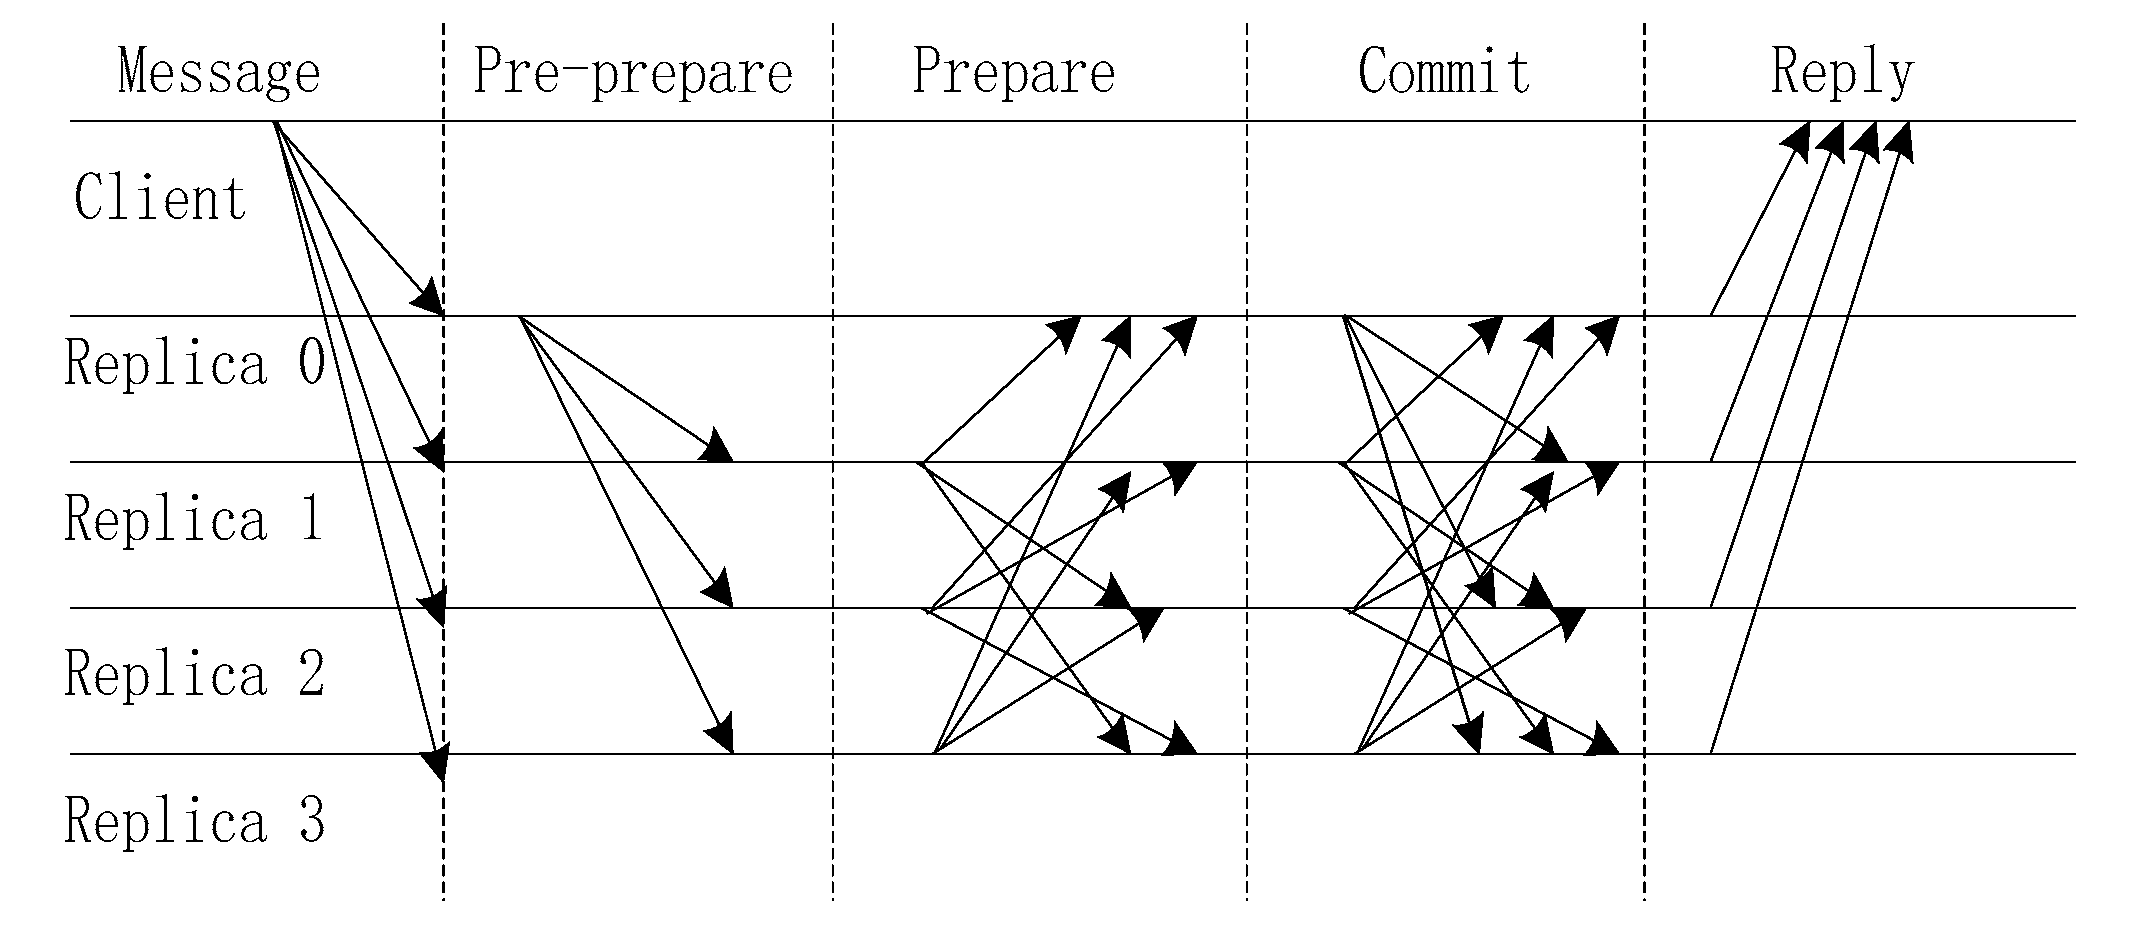
\includegraphics[width=\linewidth]{pbft-normal.png}
  \caption{PBFT-Konsensusalgorithmus im fehlerfreien Fall}
  \Description{PBFT-Konsensusalgorithmus im fehlerfreien Fall}
  \label{fig:pbft-normal}
\end{figure}

\subsection{Read-Only Optimierung}

Der Konsensusalgorithmus von PBFT hat eine hohe Nachrichtenkomplexität von $O(n^2)$. Deshalb haben die Autoren mehrere Optimierungen vorgestellt, die das PBFT-Protokoll effizienter machen sollen \cite{pbft-optimization}. Eine davon ist die Read-Only Optimierung. Sie erlaubt es Leseanfragen ohne Durchlauf des Konsensusalgorithmus beantworten zu dürfen. Die Überlegung hierbei ist, dass Leseoperationen den Zustand des Systems nicht verändern und deshalb von den Replikaten sofort ausgeführt werden sollen. Damit der Client aber keinen alten 


Die Bedingung hierfür ist allerdings wieder, dass alle vorherigen Clientanfragen sich im globalen Zustand „committed“ befinden und vom Replikat ausgeführt worden sind. Der Client wartet auf 2f+1 übereinstimmende Antworten und wiederholt die Anfrage als normale read-write Anfrage, wenn er nicht genügend Antworten innerhalb einer bestimmten Zeit erhalten hat.

\begin{figure}[htbp]
  \centering
  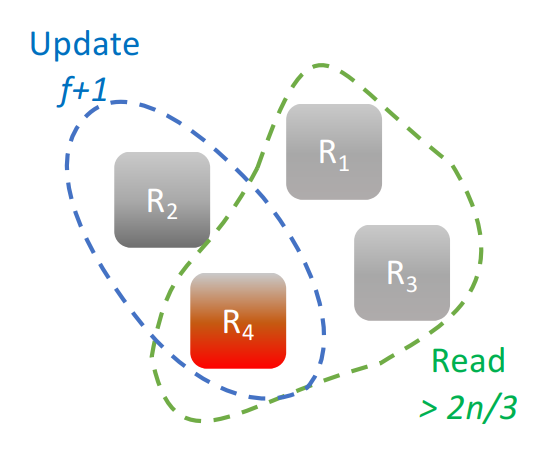
\includegraphics[width=\linewidth]{pbft-optimierung-update-quorum.png}
  \caption{Grund}
  \Description{Grund}
  \label{fig:pbft-optimization}
\end{figure}


%%
%% Print the bibliography
%%
\printbibliography

\end{document}
\endinput
